\documentclass[12pt,a4paper]{article}
\usepackage[a4paper,left=1cm,right=1cm,top=2cm,bottom=2cm]{geometry}
\usepackage{xeCJK}
\setCJKmainfont[AutoFakeBold=true]{DFKai-SB}
\usepackage{tikz}
\usepackage{tikz-3dplot}
\usetikzlibrary{patterns,patterns.meta,arrows.meta,intersections,calc,decorations.pathmorphing}
\usepackage{pgfplots}
\usepackage{amsmath}
\usepackage{amssymb}
\usepackage{float}
\usepackage{cancel}
\usepackage{fancyhdr}
\usepackage{enumitem}
\usepackage{soul}
\pgfplotsset{compat=1.18}
\setlength{\headheight}{15pt}
\newcommand \dbar {{d\mkern-6mu\mathchar'26\mkern-3mu}}
\begin{document}

\setlist[enumerate,1]{label=\textbf{\alph*.}}
\setlist[enumerate,2]{label=\roman*.} % Fallback for deeper lists

% Custom problem list environment
\newlist{problems}{enumerate}{1}
\setlist[problems]{label={}, leftmargin=0pt, itemindent=0pt}

% Modified \problem command to include underline, dash, and percentage
\newcommand{\problem}[1]{%
  \item \underline{\textbf{Problem \arabic{problemsi} -- #1}}\par\vspace{0.2cm}
}

\begin{center}
    {\large \textbf{114-2 Separation Process (分離程序) Spring, 2026}}\\[0.3cm]
    {\Large \textbf{Homework\#2}}\\[0.3cm]
    {\textbf{Post: March 12\textsuperscript{th}, 2026; Due: March 30\textsuperscript{th}, 2026}}\\[0.4cm]
    \textbf{Name: 唐麒鈞} \textbf{Student ID: B10504001}
\end{center}
\vspace{0.8cm}
\begin{problems}
\problem{Example of Terminal Velocity}
For a sedimentation process of a dilute suspension operated at 300 K, the densities of particles and fluid are 1.5 g/cm$^3$ and 1 g/cm$^3$, respectively. The fluid has a viscosity of 0.02 poise, and the suspension consists of spherical particles with a diameter of 0.08 mm.
\begin{enumerate}
    \item Calculate the terminal velocity of the suspension particles.\\
    $\rho_s$: 1.5 g/cm$^3$ = 1500 kg/m$^3$\\
    $\rho_f$: 1.0 g/cm$^3$ = 1000 kg/m$^3$\\
    $\eta$: 0.02 poise = 0.002 Pa$\cdot$s\\
    $d_{\text{sph}}$: 0.08 mm = $8\times 10^{-5}$ m\\
    Terminal velocity:
    \begin{equation}
        \nu = \frac{\left(\rho_s - \rho_f\right)gd_{\text{sph}}^2}{18\eta} =  
        \frac{(1500-1000)\cdot 9.8 \cdot \left(8\times 10^{-5}\right)^2}{18\cdot 0.002} = 8.711\times 10^{-4}~\text{m/s} 
    \end{equation}
    \# Answer: \underline{$8.711\times 10^{-4}~\text{m/s}$}
    \item Determine whether the settling falls within the Stokes' law region.
    \begin{equation}
        \text{Re}' = \frac{\rho_f \nu d_{\text{sph}}}{\eta} = \frac{1000 \cdot 8.711\times 10^{-4}\cdot 8\times 10^{-5}}{0.002} = 0.03484
    \end{equation}
    Stokes' law region: $10^{-4}< \text{Re}'<0.2$\\
    \# Answer: \underline{在 Stokes' law region裡}
\end{enumerate}
\vspace{0.2cm}
\problem{Conceptual questions}
\begin{enumerate}
    \item Define a general expression for friction factor or friction force (\textit{\textbf{F}}).
    Sketch the \textbf{drag coefficient versus Reynolds number plot} for the motion of a spherical particle in a fluid, labeling the four different zones and briefly explaining their differences.\\
    Friction force:
    \begin{equation}
        F = \begin{cases}
            3\pi \mu d u & 10^{-4}< \text{Re}' \leq 0.2\\
            3\pi \mu d u\left(1 + 0.15 \cdot \text{Re}'^{0.687}\right)  & 0.2 < \text{Re}' \leq 1000\\
            0.055 \pi d^2 \rho u^2 & 1000 < \text{Re}' \leq 2\times 10^{5} \\
            0.0125 \pi d^2 \rho u^2 & 2\times 10^{5} < \text{Re}'
        \end{cases}
    \end{equation}
    其中$u$是流體與粒子的相對速度，$d$是粒子直徑，$\rho$是流體密度，$\text{Re}'$是Particle Reynolds Number\\
    General expression，定義unit step function
    \begin{equation}
        H(x) = \begin{cases}
           0, & x <0\\
           1, & x\geq 0
        \end{cases}
    \end{equation}
    \# Answer 1:
    \begin{align}
            F =& 3\pi \mu d u \left[ H(\text{Re}' - 10^{-4}) - H(\text{Re}' - 0.2) \right] \nonumber\\
            &+ 3\pi \mu d u (1 + 0.15 \text{Re}'^{0.687}) \left[ H(\text{Re}' - 0.2) - H(\text{Re}' - 1000) \right] \nonumber\\
            &+ 0.055 \pi d^2 \rho u^2 \left[ H(\text{Re}' - 1000) - H(\text{Re}' - 2 \times 10^5) \right]\nonumber \\
            &+ 0.0125 \pi d^2 \rho u^2 H(\text{Re}' - 2 \times 10^5)
    \end{align}
    \vspace{0.2cm}
    Drag coefficient:
    \begin{equation}
        C_D = \begin{cases}
          \frac{12}{\text{Re}'} & 10^{-4}< \text{Re}' \leq 0.2\\
          \frac{12}{\text{Re}'}\left(1+0.15\cdot \text{Re}'^{0.687}\right) & 0.2 < \text{Re}' \leq 1000\\
          0.22 & 1000 < \text{Re}' \leq 2\times 10^{5} \\
          0.06 & 2\times 10^{5} < \text{Re}'
        \end{cases}
    \end{equation}
    \# Answer 2:
    \begin{figure}[H]
    \centering
    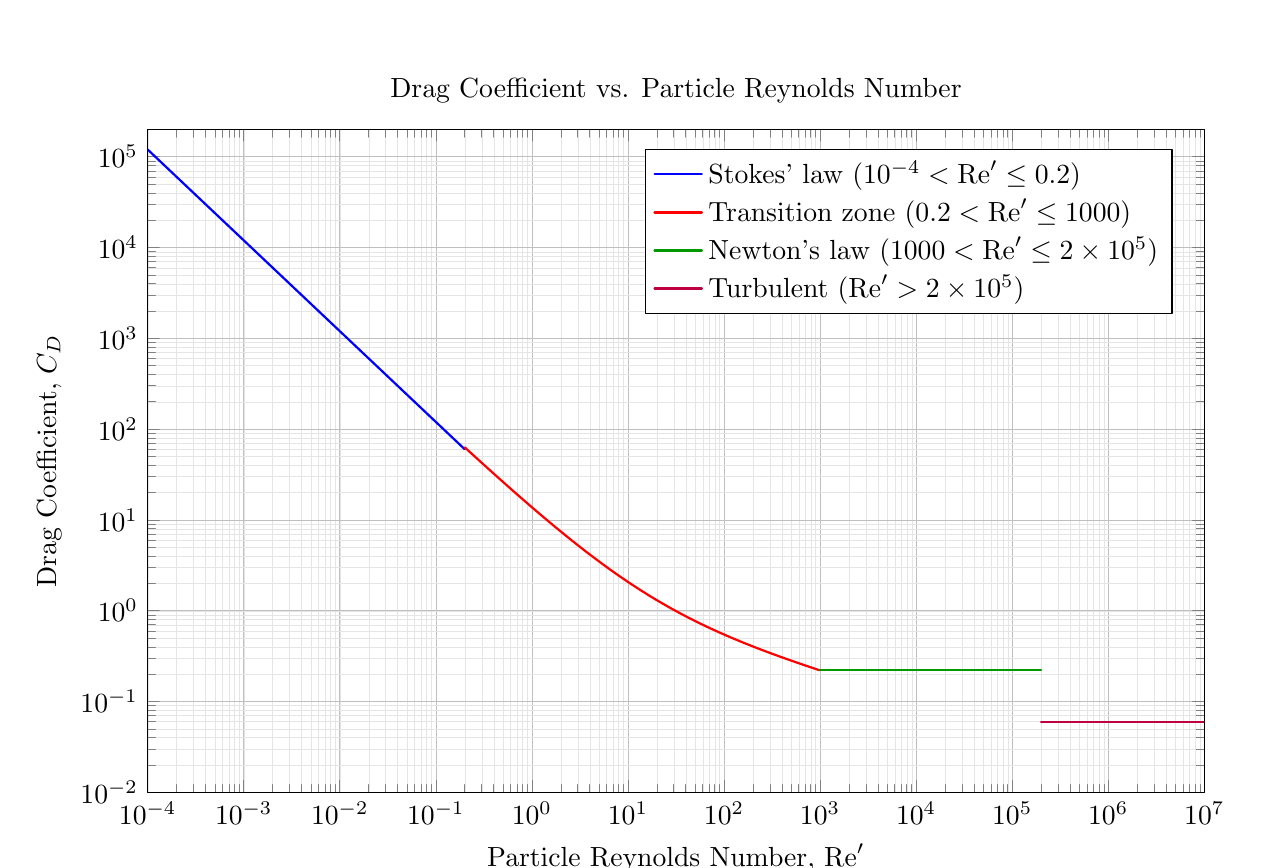
\begin{tikzpicture}[>=Latex, line cap=round, line join=round, thick]
    \begin{axis}[
        xmode=log,
        ymode=log,
        width=15cm,
        height=10cm,
        grid=both,
        grid style={line width=.1pt, draw=gray!20},
        major grid style={line width=.2pt, draw=gray!50},
        xlabel={Particle Reynolds Number, $\text{Re}'$},
        ylabel={Drag Coefficient, $C_D$},
        xmin=1e-4, xmax=1e7,
        ymin=1e-2, ymax=2e5,
        legend pos=north east,
        legend cell align=left,
        title={Drag Coefficient vs. Particle Reynolds Number},
        % This forces scientific notation for the axis labels
        log basis x={10},
        log basis y={10}
    ]
    
    % Region 1: Stokes Regime
    \addplot [
        domain=1e-4:0.2,
        samples=50,
        thick,
        blue
    ] {12/x};
    \addlegendentry{Stokes' law ($10^{-4} < \text{Re}' \le 0.2$)}
    
    % Region 2: Transition Regime
    \addplot [
        domain=0.2:1000,
        samples=500,
        thick,
        red
    ] {12/x * (1 + 0.15 * x^(0.687596944))};
    \addlegendentry{Transition zone ($0.2 < \text{Re}' \le 1000$)}
    
    % Region 3: Newtonian Regime
    \addplot [
        domain=1000:200000, % 2 * 10^5
        samples=10,
        thick,
        green!60!black
    ] {0.22};
    \addlegendentry{Newton's law ($1000 < \text{Re}' \le 2\times 10^5$)}
    
    \addplot [
        domain=200000:1e7, % Extended to 10^7 for visual completion
        samples=10,
        thick,
        purple
    ] {0.06};
    \addlegendentry{Turbulent ($\text{Re}' > 2\times 10^5$)}
    
    \end{axis}
    \end{tikzpicture}
    \caption{Drag coefficient versus Reynolds number plot}
    \end{figure}
    \# Answer 3\\
    這四個區域的主要差別在於流體繞過粒子時，黏滯力與慣性力的重要性不同
    \begin{itemize}
        \item Stokes' law:\\
        粒子周圍的流動非常平穩，流體的黏滯力遠大於慣性力，沒有明顯的流線分離\\
        阻力主要來自流體的黏滯剪應力，故與雷諾數成反比
        \item Transition zone:\\
        流體的慣性力開始變得不可忽略，阻力係數多加上了一個$0.15 \text{Re}'^{0.687}$的修正\\
        代表流場開始由純黏滯控制，逐漸過渡到慣性控制。
        \item Newton's law:\\
        慣性力主導，壓力成為阻力主要來源，故此時阻力係數為常數。\\
        與下個區間的差別在於粒子後方會形成穩定的尾流與流線分離
        \item Turbulent regime:\\
        與上個區間的差別在於\\
        粒子周圍邊界層變成紊流，使得分離點延後，
        使得尾流變小，阻力下降。
    \end{itemize}
    \item Define the \textbf{apparent settling velocity (\textit{u\textsubscript{c}})} and relative velocity (particle velocity relative to fluid velocity, \textit{\textbf{u\textsubscript{p}}}). Describe their relationship using \textbf{voidage (\textit{e})}.\\
    \# Answer:
    \begin{itemize}
        \item Apparent settling velocity $u_c$:\\
        粒子相對於\fbox{容器}的下降速度
        \item Relative velocity $u_p$:\\
        粒子相對於\fbox{流體}的速度
        \item Voidage $e$:\\
        系統中流體所占的體積分率，反過來說粒子的體積分率為$1-e$\\
        在截面固定下，若沒有真空，當固體向下移動時，流體必須向上補因此
        \begin{equation}
            (1-e)u_c + e(-u_f) = 0,~ u_f\text{是液體相對於容器的速度，與粒子速度相反} \label{eq1}
        \end{equation}
        因此相對速度可寫為:
        \begin{equation}
            u_p = u_c + u_f
        \end{equation}
        代入(\ref{eq1})
        \begin{equation}
            (1-e)u_c - e(u_p-u_c)= 0 \implies u_c - eu_p = 0
        \end{equation}
        移項後得到:
        \begin{equation}
            \underline{u_c = e u_p}
        \end{equation}
    \end{itemize}
\end{enumerate}
\problem{Example of a rotary drum}
A rotary drum filter, with a diameter of 2 m and a length of 2.5 m, operates with 25\% of its
surface immersed in the slurry and under a vacuum of 100 kPa.
The slurry to be filtered contains 50\% solids by mass of density 2,500 kg/$\text{m}^3$.
A laboratory test on a sample of the slurry, 
a leaf filter with a filtration area of 100 cm$^2$, covered with a cloth similar to the one
used on the drum, produced 220 cm$^3$ of filtrate in the first minute and 110 cm$^3$ of filtrate in
the next minute when subjected to a vacuum of 10 kPa. The bulk density of the wet cake was
2,000 kg/m$^3$, and the density of the filtrate was 1,000 kg/m$^3$. The cake is assumed to be
incompressible, and a 5 mm thick layer of cake remains on the drum after filtration.
\begin{enumerate}
    \item Determine the \textbf{voidage ($\boldsymbol{\varepsilon}$)} of the wet cake.\\
    質量守恆
    \begin{equation}
        \rho_{c,\text{wet}}=(1-\varepsilon)\rho_s+\varepsilon\rho_f
    \end{equation}
    \begin{equation}
        2000=(1-\varepsilon)(2500)+\varepsilon(1000)
    \end{equation}
    \begin{equation}
        2000=2500-1500\varepsilon
        \;\Rightarrow\;
        \varepsilon=\frac{2500-2000}{1500}=0.333
    \end{equation}
    \# Answer: \underline{$\varepsilon=0.333$}
    \item Determine the volume of cake deposited by \textbf{unit volume of filtrate ($\boldsymbol\nu$)}.\\
    假設有1 kg slurry. 因為slurry含有50 wt\%固體:
    \begin{equation}
        m_s=0.5~\text{kg},\qquad m_f=0.5~\text{kg}
    \end{equation}
    固體體積:
    \begin{equation}
        V_s=\frac{m_s}{\rho_s}=\frac{0.5}{2500}=2.0\times10^{-4}~\text{m}^3
    \end{equation}
    Wet cake體積:\\
    因為cake中固體只占$(1-\varepsilon)$，所以
    \begin{equation}
        V_c=\frac{V_s}{1-\varepsilon}
        =\frac{2.0\times10^{-4}}{1-0.333}
        =3.0\times10^{-4}~\text{m}^3
    \end{equation}
    Cake 中保留的液體體積
    \begin{equation}
        V_{f,\text{in cake}}=\varepsilon V_c
        =(0.333)(3.0\times10^{-4})
        =1.0\times10^{-4}~\text{m}^3
    \end{equation}
    初始液體體積
    \begin{equation}
        V_{f,\text{initial}}=\frac{m_f}{\rho_f}=\frac{0.5}{1000}=5.0\times10^{-4}~\text{m}^3
    \end{equation}
    因此過濾掉的液體體積
    \begin{equation}
        V_{f,\text{filtered}}=V_{f,\text{initial}}-V_{f,\text{in cake}}=5.0\times10^{-4}-1.0\times10^{-4}=4.0\times10^{-4}~\text{m}^3
    \end{equation}
    因此每過濾掉1 m$^3$的液體，會形成的cake體積為
    \begin{equation}
        \nu=\frac{V_c}{V_{f,\text{filtered}}}=\frac{3.0\times10^{-4}}{4.0\times10^{-4}}=0.75~\text{m}^3_{\text{cake}}/\text{m}^3_{\text{filtrate}}
    \end{equation}
    \# Answer: \underline{$\nu=0.75~\text{m}^3_{\text{cake}}/\text{m}^3_{\text{filtrate}}$}
    \item Determine the \textbf{equivalent thickness ($\boldsymbol{L}$)} caused by the filter cloth and support.\\
    在Constant Pressure下，考慮filter cloth + support時:
    \begin{equation}
      V^2 + \frac{2LA}{\nu}V = \frac{2A^2\left|\Delta P\right|}{\mu\gamma\nu}t \label{eq8}
    \end{equation}
    同除以$V$，並整理:
    \begin{align}
      V  + \frac{2LA}{\nu} =& \frac{2A^2\left|\Delta P\right|}{\mu\gamma\nu}\frac{t}{V} \nonumber\\
      \mu\gamma\nu V + 2\mu\gamma LA =& 2A^2\left|\Delta P\right|\frac{t}{V} \nonumber\\
      \frac{t}{V} &= \boxed{\frac{\mu\gamma\nu}{2A^2\left|\Delta P\right|}}V + \boxed{\frac{\mu\gamma L}{A\left|\Delta P\right|}} \label{eq2}
    \end{align}
    令:
    \begin{equation}
        m=\frac{\mu\gamma\nu}{2A^2\left|\Delta P\right|},\qquad b=\frac{\mu\gamma L}{A\left|\Delta P\right|} \label{eq6}
    \end{equation}
    使得:
    \begin{equation}
        \frac{t}{V} = mV + b \label{eq3}
    \end{equation}
    而$b/m$為:
    \begin{equation}
      \frac{b}{m} = \frac{\frac{\mu\gamma L}{A\left|\Delta P\right|}}{\frac{\mu\gamma\nu}{2A^2\left|\Delta P\right|}} = \frac{2LA}{\nu}
    \end{equation}
    移項可得到$L$:
    \begin{equation}
      L = \frac{b}{m}\cdot \frac{\nu}{2A} \label{eq5}
    \end{equation}
    由實驗數據可得兩點:
    \begin{itemize}
      \item 第1分鐘後:
      \begin{equation}
        t_1 = 1 \text{ min}  = 60 \text{ s},\qquad V_1 = 220 \text{ cm}^3 = 2.2\times10^{-4} \text{ m}^3
      \end{equation}
      \item 第2分鐘後:
      \begin{equation}
        t_2 = 2 \text{ min}  = 120 \text{ s},\qquad V_2 = 220 + 110 = 330 \text{ cm}^3 = 3.3\times10^{-4} \text{ m}^3
      \end{equation}
    \end{itemize}
    將兩點代入(\ref{eq3})，得到兩條方程式:
    \begin{equation}
      \begin{cases}
        \frac{60}{2.2\times10^{-4}} = m(2.2\times10^{-4}) + b \\
        \frac{120}{3.3\times10^{-4}} = m(3.3\times10^{-4}) + b
      \end{cases}\label{eq4}
    \end{equation}
    將兩式相減:
    \begin{align}
      &\frac{120}{3.3\times10^{-4}} - \frac{60}{2.2\times10^{-4}} = m\left(3.3\times10^{-4} - 2.2\times10^{-4}\right) \\
      \implies&
      m = \frac{\frac{120}{3.3\times10^{-4}} - \frac{60}{2.2\times10^{-4}}}{3.3\times10^{-4} - 2.2\times10^{-4}} = 8.264\times10^8~\text{s/m}^6
    \end{align}
    代回(\ref{eq4})的第一式，解出$b$:
    \begin{equation}
      \frac{60}{2.2\times10^{-4}} = (8.264\times10^8)(2.2\times10^{-4}) + b \implies b = 9.0919\times10^4~\text{s/m}^3
    \end{equation}
    代入(\ref{eq5}):\\
    100 cm$^2$ = 0.01 m$^2$
    \begin{equation}
      L = \frac{9.0919\times10^4}{8.264\times10^8}\cdot \frac{0.75}{2\cdot 0.01} = 4.12568\times 10^{-3}~\text{m}
    \end{equation}
    \# Answer: \underline{$L=4.126\times10^{-3}~\text{m}=4.126~\text{mm}$}
    \item Determine the \textbf{specific resistance ($\boldsymbol{\gamma}$)} of the filter cake if the viscosity of the filtrate is 0.001 Pa$\cdot$s.\\
    由剛剛(\ref{eq6})的$m$，求出$\gamma$:\\
    $\left|\Delta P\right|=10~\text{kPa}=10^4~\text{Pa}$
    \begin{equation}
      m = \frac{\mu\gamma\nu}{2A^2\left|\Delta P\right|} \implies \gamma = \frac{2A^2\left|\Delta P\right|m}{\mu\nu} = 
      \frac{2\cdot 0.01^2\cdot 10^4\cdot 8.264\times10^8}{0.001\cdot 0.75} = 2.2037\times10^{12}~\text{m}^{-2}
    \end{equation}
    \# Answer: \underline{$\gamma=2.2037\times10^{12}~\text{m}^{-2}$}
    \item Estimate the diameter of the particles if the slurry consists of uniform spherical particles.\\
    由Carman-Kozeny relation:
    \begin{equation}
      \gamma = \frac{5S^2\left(1-\varepsilon\right)^2}{\varepsilon^3} \label{eq7}
    \end{equation}
    假設粒子是uniform spherical particles，則比表面積$S$為:
    \begin{equation}
      S = \frac{6}{d_p}
    \end{equation}
    代回(\ref{eq7}):
    \begin{equation}
      \gamma = \frac{5\left(\frac{6}{d_p}\right)^2\cdot\left(1-\varepsilon\right)^2}{\varepsilon^3} = \frac{180\left(1-\varepsilon\right)^2}{\varepsilon^3 d_p^2}
    \end{equation}
    整理可得:
    \begin{equation}
      d_p^2 = \frac{180\left(1-\varepsilon\right)^2}{\varepsilon^3 \gamma} \implies d_p = \sqrt{\frac{180\left(1-\varepsilon\right)^2}{\varepsilon^3 \gamma}}
    \end{equation}
    將$\gamma=2.2037\times10^{12}~\text{m}^{-2}$, $\varepsilon=0.333$代入:
    \begin{equation}
      d_p =\sqrt{
        \frac{180\left(1-0.333\right)^2}{0.333^3 \cdot 2.2037\times10^{12}}
      } = 3.137 \times 10^{-5}~\text{m}
    \end{equation}
    \# Answer: \underline{$d_p=3.137\times10^{-5}~\text{m}\approx 31.3~\mu \text{m}$}
    \item Determine the drum speed required to achieve a filtration rate of 50\% of the maximum filtration rate.\\
    由於在Drum上除了Filter cloth+support的阻力外，還有一個5 mm厚的cake層的阻力\\
    因此在Constant Pressure下，總固定阻力的厚度為:
    \begin{equation}
      L_{\text{total}} = L + 0.005~\text{m} = 0.00412568 + 0.005 = 0.00912568~\text{m}
    \end{equation}
    將(\ref{eq8})中的$L$換成$L_{\text{total}}$，並將$V$換成$V_{\text{max}}$，得到最大過濾率的方程式:
    \begin{equation}
      V_{\text{max}}^2 + \frac{2L_{\text{total}}A}{\nu}V_{\text{max}} = \frac{2A^2\left|\Delta P\right|}{\mu\gamma\nu}t \label{eq9}
    \end{equation}
    同除以$A^2$:
    \begin{equation}
      \left(\frac{V_{\text{max}}}{A}\right)^2 + \frac{2L_{\text{total}}}{\nu}\frac{V_{\text{max}}}{A} = \frac{2\left|\Delta P\right|}{\mu\gamma\nu}t \label{eq10}
    \end{equation}
    令$w=\frac{V_{\text{max}}}{A}$，則(\ref{eq10})可寫為:
    \begin{equation}
      w^2 + \frac{2L_{\text{total}}}{\nu}w = \frac{2\left|\Delta P\right|}{\mu\gamma\nu}t \label{eq11}
    \end{equation}
    由於Drum已經有25\%的表面積浸在slurry裡，所以每一轉中，只有25\%的時間在過濾
    \begin{equation}
      t_f = 0.25 T
    \end{equation}
    其中$T$是轉一圈的時間，$T=\frac{1}{N}$，$N$是轉速(轉/s)。\\
    因此(\ref{eq11})可寫為:
    \begin{equation}
      w^2 + \frac{2L_{\text{total}}}{\nu}w = \frac{2\left|\Delta P\right|}{\mu\gamma\nu}\cdot 0.25 \cdot \frac{1}{N} \label{eq12}
    \end{equation}
    由(\ref{eq12})可解出$w$:
    \begin{align}
      &w^2 + \frac{2L_{\text{total}}}{\nu}w - \frac{2\left|\Delta P\right|}{\mu\gamma\nu}\cdot 0.25 \cdot \frac{1}{N} = 0 \nonumber\\
      \implies w =& \frac{
      -\frac{2L_{\text{total}}}{\nu} \pm \sqrt{\left(\frac{2L_{\text{total}}}{\nu}\right)^2 + 4\cdot \frac{2\left|\Delta P\right|}{\mu\gamma\nu}\cdot 0.25 \cdot \frac{1}{N}}}{2} \nonumber\\
      \text{取正值}\implies w =& 
      \frac{-\frac{2L_{\text{total}}}{\nu} + \sqrt{\left(\frac{2L_{\text{total}}}{\nu}\right)^2 + 4\cdot \frac{2\left|\Delta P\right|}{\mu\gamma\nu}\cdot 0.25 \cdot \frac{1}{N}}}{2} \nonumber\\
      =& \frac{-2L_{\text{total}}}{\nu} + \sqrt{
        \left(\frac{L_{\text{total}}}{\nu}\right)^2 + \frac{0.5\left|\Delta P\right|}{\mu\gamma\nu}\cdot \frac{1}{N}
      } \label{eq13}
    \end{align}
    令
    \begin{equation}
      B = \frac{L_{\text{total}}}{\nu},\qquad K = \frac{0.5\left|\Delta P\right|}{\mu\gamma\nu}
    \end{equation}
    則(\ref{eq13})可寫為:
    \begin{equation}
      w = -B + \sqrt{B^2 + \frac{K}{N}} \label{eq14}
    \end{equation}
    定義Filtration rate per area ($Q$):
    \begin{equation}
      Q = Nw
      = N\left(-B + \sqrt{B^2 + \frac{K}{N}}\right)
    \end{equation}
    代入(\ref{eq14})的$w$，得到$Q$的表達式:
    \begin{equation}
      Q = N\left(-B + \sqrt{B^2 + \frac{K}{N}}\right) \label{eq15}
    \end{equation}
    整理:
    \begin{align}
      Q &= N\left(\sqrt{B^2+\frac{K}{N}}-B\right) \nonumber\\
        &= N\cdot\frac{\left(B^2+\frac{K}{N}\right)-B^2}{\sqrt{B^2+\frac{K}{N}}+B} \nonumber\\
        &= N\cdot\frac{K/N}{\sqrt{B^2+\frac{K}{N}}+B} \nonumber\\
        &= \frac{K}{\sqrt{B^2+\frac{K}{N}}+B}
    \end{align}
    當$N\to\infty$時，$\frac{K}{N}\to 0$，因此最大過濾速率為
    \begin{equation}
      Q_{\max} = \frac{K}{2B}
    \end{equation}
    題目要求過濾速率為最大過濾速率的50\%，故
    \begin{equation}
      Q = \frac{1}{2}Q_{\max} = \frac{K}{4B}
    \end{equation}
    因此
    \begin{align}
      &\frac{K}{\sqrt{B^2+\frac{K}{N}}+B} = \frac{K}{4B} \nonumber\\
      \implies & \frac{1}{\sqrt{B^2+\frac{K}{N}}+B} = \frac{1}{4B} \nonumber\\
      \implies & \sqrt{B^2+\frac{K}{N}}+B = 4B \nonumber\\
      \implies & \sqrt{B^2+\frac{K}{N}} = 3B \nonumber\\
      \implies & B^2+\frac{K}{N} = 9B^2 \nonumber\\
      \implies & \frac{K}{N} = 8B^2 \nonumber\\
      \implies & N = \frac{K}{8B^2}
    \end{align}
    代入$B$的定義:
    \begin{equation}
      B = \frac{L_{\text{total}}}{\nu} = \frac{0.00912568}{0.75} = 0.01216757~\text{m}
    \end{equation}
    代入$K$的定義\\
    操作時的壓力差$\left|\Delta P\right|$為100 kPa = $10^5$ Pa，黏度$\mu$為0.001 Pa$\cdot$s，則
    \begin{equation}
      K = \frac{0.5\left|\Delta P\right|}{\mu\gamma\nu} = 
      \frac{0.5\cdot 10^5}{0.001\cdot 2.2037\times10^{12}\cdot 0.75} = 3.025\times10^{-5}~\text{m/s}
    \end{equation}
    因此轉速為:
    \begin{equation}
      N = \frac{K}{8B^2} = \frac{3.025\times10^{-5}}{8\cdot (0.01216757)^2} = 0.0255~\text{轉/s}
    \end{equation}
    最後將轉速換算成rpm:
    \begin{equation}
      N = 0.0255~\text{轉/s} \cdot 60~\text{s/min} = 1.53~\text{rpm}
    \end{equation}
    \# Answer: \underline{$N\approx 1.53~\text{rpm}$}
\end{enumerate}
\end{problems}
\end{document}
